\section{Introduction}
\label{sec:section}
  Keyphrases are single or multi-word expressions that represent the main topics
  of a document. Keyphrases are useful in many tasks such as information
  retrieval~\cite{medelyan2008smalltrainingset}, document
  summarization~\cite{litvak2008graphbased} or document
  clustering~\cite{han2007webdocumentclustering}. Although scientific articles
  usually provide them, most of the documents have no associated keyphrases.
  Therefore, the problem of automatically assigning keyphrases to documents is
  an active field of research.

  Automatic keyphrase extraction methods are divided into two categories:
  supervised and unsupervised methods. Supervised methods typically recast
  keyphrase extraction as a binary classification
  task~\cite{witten1999kea,sujian2003maximumentropy,eichler2010keywe}. For
  unsupervised methods, keyphrase extraction is often considered as a ranking
  task and many approaches are
  used~\cite{barker2000nounphrasehead,mihalcea2004textrank}. Although they work
  diferently, both supervised and unsupervised methods rely on a preliminary
  candidate extraction step which identifies single and multi-word expressions
  that have the same syntactic properties than a keyphrase. These expressions
  are the only textual units that can be extracted as keyphrases. Therefore, we
  believe that the extraction of candidate keyphrases plays a direct role in
  automatic keyphrase extraction.
  
  In this paper, we focus on the candidate extraction step and show its impact
  on the performance of automatic keyphrase extraction. Various methods
  are commonly employed to extract keyphrase candidates\footnote{In this work,
  we do not consider methods which use a manually defined controlled
  vocabulary.}. Usually, a set of either single words, n-grams filtered by stop
  words, NP-chunks or sequences of words matching given patterns is
  extracted~\cite{hulth2003keywordextraction}. According to the chosen method,
  the extracted set contains more or less candidates, and the amount of these
  that are actual keyphrases may vary. Hence, a few questions arise. How the
  different sets influence the keyphrase extraction? Do large candidate sets
  introduce noise that affects the performance of some keyphrase extraction
  methods?

  We seek to better understand the impact of candidate extraction methods on
  keyphrase extraction by studying the aforementioned questions. We first
  quantify the differences between the candidate sets obtained by the commonly
  used methods and we propose to use other methods developed for automatic term
  detection~\cite{castellvi2001automatictermdetection,evans1996nounphraseanalysis}
  to show that such methods provide solid keyphrase candidates. Then, we
  evaluate the impact of the candidate extraction methods over three dissimilar
  keyphrase extraction methods. We select KEA~\cite{witten1999kea} to represent
  supervised methods, TF-IDF~\cite{jones1972tfidf} to represent unsupervised
  methods that require a collection of documents and
  TopicRank~\cite{bougouin2013topicrank} to represent unsupervised methods that
  only make use of the analyzed document.

  \todo[inline]{Results show that...}

\section{Definition of Candidate Keyphrases}
\label{sec:study_of_ground_truth_keyphrases}
  Candidate keyphrases are textual units which can be selected as keyphrases
  of a document. Hence, they must have the same syntactic and linguistic
  properties than ground truth keyphrases. This section aims to determine those
  properties by analysing three standard evaluation datasets, for keyphrase
  extraction, and by providing statistics about their reference keyphrases
  (ground truth keyphrases).

  \subsection{Keyphrase Extraction Datasets}
  \label{subsec:keyphrase_extraction_datasets}
    Keyphrase extraction datasets are used to train or evaluate keyphrase
    extraction methods. Hence, they are collections of documents paired with
    reference keyphrases given by authors, readers or both. Unlike the methods
    to automatically extract keyphrases, human annotators do not only provide
    keyphrases contained into the documents. This problem of missing keyphrases
    leads to a bias of the training or evaluation of keyphrase extraction
    methods. In this work, we use three standard datasets which differ in terms
    of document size,  type and language. The problem of missing keyphrases is
    partially bypassed using stemmed forms when comparison between reference and
    candidate keyphrases is needed.

    The \textbf{DUC} dataset \cite{over2001duc} is a collection of 308 English
    news articles covering about 30 topics (e.g. tornadoes, gun control, etc.).
    This collection is the test dataset of the DUC-2001 summarization evaluation
    campaign. This part of DUC-2001 is the only one that contains keyphrases,
    annotated by \newcite{wan2008expandrank}. We split the collection into two
    sets: a training set containing 208 documents and a test set containing 100
    documents.

    The \textbf{SemEval} dataset \cite{kim2010semeval} contains 284 English
    papers collected from the ACM Digital Libraries (conference and workshop
    papers). The papers are divided into three sets: a trial set containing 40
    documents (unused in this work), a training set containing 144 documents and
    a test set containing 100 documents. As for the associated keyphrases, these
    are provided by both authors and readers.

    The \textbf{DEFT} dataset \cite{Paroubek2012deft} is a collection of 234
    French scientific papers belonging to the Humanities and Social Sciences
    domain. DEFT is divided into two sets: a training set containing 141
    documents and a test set containing 93 documents. The only available
    reference keyphrases are the ones given by authors.

    Table \ref{tab:train_dataset_statistics} shows the statistics about the
    three datasets. As these statistics are used to guide our work, we restrain
    them to the training sets. As said before, the datasets differ in terms of
    size, type and language. Moreover, it is worth noticing that the number of
    keyphrases, the ratio of missing ones and the average number of tokens per
    keyphrases differ too. These are due to the fact that there is not a unique
    methodology (guideline) to manually associate keyphrases to a document. To
    better fit the requirements, such guidelines should not only be used by
    human annotators, but also by automatic keyphrase extraction methods.
    \todo{[CAPTION] Others are mainly foreign words and coordinating conjonctions.}
    \begin{table*}
      \centering
      \begin{tabular}{rrccc}
        \toprule
        & \multirow{2}{*}[-2pt]{\textbf{Statistics}} & \multicolumn{3}{c}{\textbf{Corpora}}\\
        \cmidrule{3-5}
        & & DUC & SemEval & DEFT\\
        \midrule
        \multirow{6}{*}[-2pt]{\begin{sideways}\textbf{Documents}\end{sideways}} & Language & English & English & French\\
        & Type & News & Papers & Papers\\
        & Documents & 208 & 144 & 141\\
        & Tokens/document & 912.0 & 5134.6 & 7276.7\\
        & Keyphrases/document & 8.1 & 15.4 & 5.4\\
        & Missings keyphrases & 3.9\% & 13.5\% & 18.2\%\\
        \addlinespace[1.5\defaultaddspace]
        \multirow{5}{*}[-2pt]{\begin{sideways}\textbf{Keyphrases}\end{sideways}} & Unigrams & 17.1\% & 20.2\% & 60.2\%\\
        & Bigrams & 60.8\% & 53.4\% & 24.5\%\\
        & Trigrams & 17.8\% & 21.3\% & $~~$8.8\%\\
        & Quadrigrams & $~~$3.0\% & $~~$3.9\% & $~~$4.2\%\\
        & N-grams (N $\geq$ 5) & $~~$1.3\% & $~~$1.3\% & $~~$2.4\%\\
        \addlinespace[1.5\defaultaddspace]
        \multirow{5}{*}[-2pt]{\begin{sideways}\textbf{Multi-word keyphrases}\end{sideways}} & Containing nouns & 94.5\% & 98.7\% & 93.3\%\\
        & Containing proper nouns & 17.1\% & $~~$4.3\% & $~~$6.9\%\\
        & Containing adjectives & 50.0\% & 50.2\% & 65.5\%\\
        & Containing verbs & $~~$1.0\% & $~~$4.0\% & $~~$1.0\%\\
        & Containing adverbs & $~~$1.6\% & $~~$0.7\% & $~~$1.3\%\\
        & Containing prepositions & $~~$0.3\% & $~~$1.5\% & 31.2\%\\
        & Containing determiners & $~~$0.0\% & $~~$0.0\% & $~~$20.4\%\\
        & Containing others & $~~$1.5\% & $~~$2.5\% & $~~$11.8\%\\
        \addlinespace[.5\defaultaddspace]
        \bottomrule
      \end{tabular}
      \caption{Training dataset statistics. As a matter of consistency regarding
               the training and the evaluation of keyphrase extraction methods,
               the percentage of missing keyphrases is determined based on the
               stemmed form of the reference keyphrases.
               \label{tab:train_dataset_statistics}}
    \end{table*}

  \subsection{Reference Keyphrases Analysis}
  \label{subsec:keyphrase_analysis}
    Despite the fact that the data are not homogeneous, this section aims to
    find the syntactic properties of most keyphrases, for English (intersecting
    information from DUC and SemEval) and for French (using DEFT). To avoid from
    biasing our work we only exploit information from the training data.

    The first observation from Table \ref{tab:train_dataset_statistics} is that
    most of the keyphrases are unigrams or bigrams ($\simeq$~80\%). This, plus
    the fact that the number of n-gram keyphrases (n $\geq$ 3) decrease when n
    increase, means that keyphrases are more often less informative. Keyphrases
    bear the minimum information to represent one important idea (e.g. TODO
    instead of TODO).

    \begin{itemize}
      \item{About 80\% of reference keyphrases contain only one or two words.}
      \item{Toutes les keyphrases de référence ont étées POS tagguées
            automatiquement, puis vérifiées manuellement, afin d'obtenir les
            stats du tableau 1.}
      \item{Almost every keyphrases contain nouns or proper nouns.}
      \item{Adjective modifiers are almost the only other compounds of
            keyphrases, except for French where prepositionnal phrases are
            used.}
    \end{itemize}
    \todo[inline]{\begin{center}DONNER DES EXEMPLES\end{center}}
    \todo[inline]{Donner les séquences de POS les plus fréquentes dans le gold
                  standard.}
    \paragraph{English:} NOUN NOUN (huricane expert -- AP880409-0015); ADJ NOUN
    (turbulent summer -- AP880409-0015); NOUN (storms -- AP880409-0015); ADJ
    NOUN NOUN (annual huricane forecast -- AP880409-0015); NOUN NOUN NOUN
    (huricane reconnaissance -- AP890529-0030).
    \paragraph{French:} NOUN (patrimoine -- as\_2002\_007048ar); NOUN ADJ
    (tradition orale -- as\_2002\_007048ar); PROPER NOUN (Indonésie --
    as\_2001\_000235ar); NOUN PREP DET NOUN (conservation de la nature --
    as\_2005\_011742ar); NOUN PREP NOUN (changement de terrain --
    as\_2001\_000260ar).

\section{Candidate Extraction}
\label{sec:candidate_extraction}
  \todo[inline]{Objectif + pré-requis.}

  \subsection{N-Gram Extraction}
  \label{subsec:n_gram_extraction}

  \subsection{NP-Chunk Extraction}
  \label{subsec:np_chunk_extraction}
    \paragraph{English:} (PROPER NOUN+) $|$ (ADJ+ NOUN) $|$ (NOUN+)
    \paragraph{French:} (PROPER NOUN+) $|$ (ADJ? NOUN ADJ+) $|$ (ADJ NOUN) $|$ (NOUN+)

  \subsection{Pattern Matching}
  \label{subsec:pattern_matching}
    \paragraph{Longest NP:} (NOUN $|$ ADJ)+
    \paragraph{English:} (NOUN\{1, 3\}) $|$ (ADJ NOUN\{1, 2\}) $|$ ((NOUN $|$ ADJ) ADJ NOUN) $|$ (PROPER NOUN (PROPER NOUN $|$ NOUN)?)
    \paragraph{French:} (NOUN (PREP DET? NOUN)? ADJ?) $|$ (PROPER NOUN+)

  \subsection{Term Extraction}
  \label{subsec:term_extraction}

\section{Keyphrase Extraction}
\label{sec:keyphrase_extraction}
  \todo[inline]{Fonctionnement général.}
  \begin{figure}
    \centering
    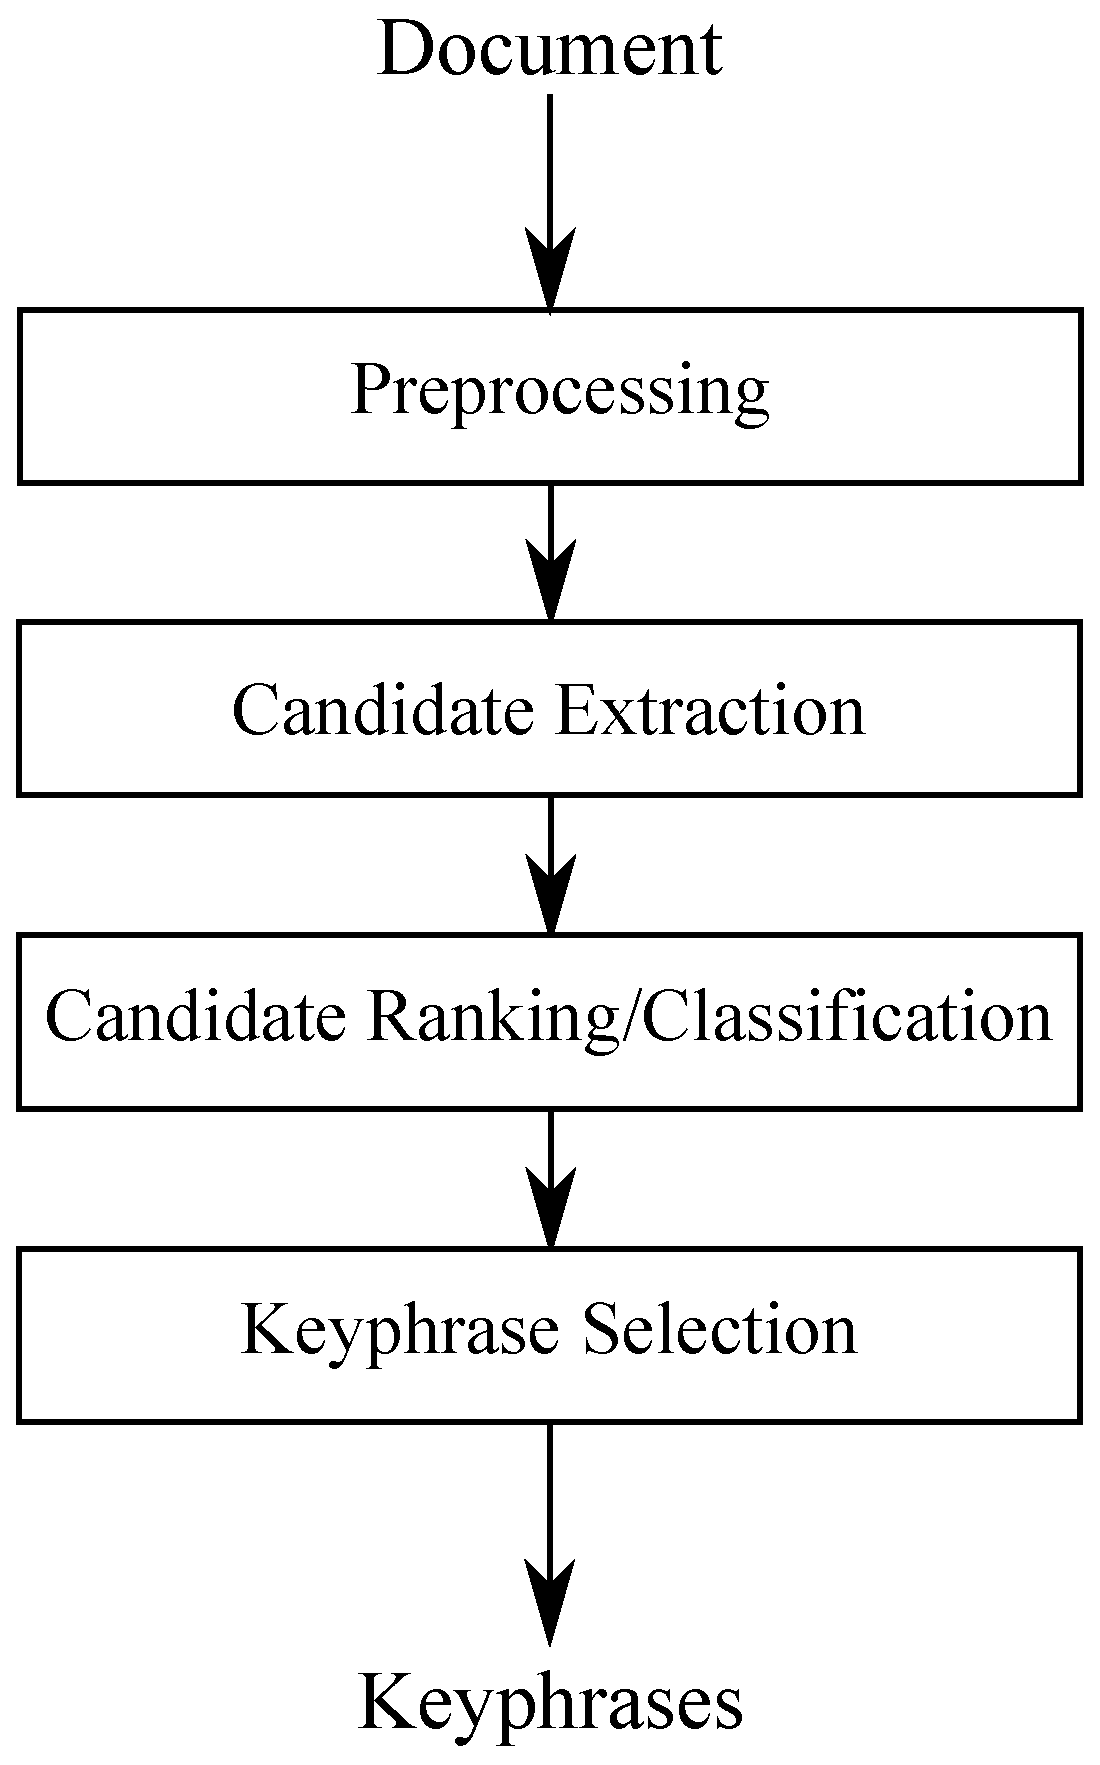
\includegraphics[width=0.3\textwidth]{include/processing_steps.eps}
    \caption{Processing steps of automatic keyphrase extraction methods.
             \label{fig:processing_steps}}
  \end{figure}

  \subsection{TF-IDF}
  \label{subsec:tfidf}
  \subsection{TopicRank}
  \label{subsec:topicrank}
  \subsection{KEA}
  \label{subsec:kea}

\section{Evaluation}
\label{sec:evaluation}
  \todo[inline]{Expliquer les deux évaluations: intrinsèque et extrinsèque.}

  \subsection{Experimental Setting}
  \label{subsec:experimental_setting}
    \begin{table*}
      \centering
      \begin{tabular}{rccc}
        \toprule
        \multirow{2}{*}[-2pt]{\textbf{Statistics}} & \multicolumn{3}{c}{\textbf{Corpora}}\\
        \cmidrule{2-4}
        & DUC & SemEval & DEFT\\
        \midrule
        Language & English & English & French\\
        Type & News & Papers & Papers\\
        Documents & 100 & 100 & 93\\
        Tokens/document & 877.3 & 5177.7 & 6839.4\\
        Keyphrases/document & 7.94 & 14.7 & 5.2\\
        Tokens/keyphrase & 2.1 & 2.1 & 1.6\\
        Missings keyphrases & 2.8\% & 22.1\% & 21.1\% \\
        \bottomrule
      \end{tabular}
      \caption{Test dataset statistics. As a matter of consistency regarding
               the training and the evaluation of keyphrase extraction methods,
               the percentage of missing keyphrases is determined based on the
               stemmed form of the reference keyphrases.
               \label{tab:test_dataset_statistics}}
    \end{table*}

  \subsection{Candidate Extraction}
  \label{subsec:candidate_extraction}
    \todo[inline]{Donner le rappel max et comparer avec la taille des différents
                  ensemble.}

    \begin{table*}[h]
      \centering
      \begin{tabular}{rcccccc}
        \toprule
        \multirow{2}{*}[-2pt]{\textbf{Methods}} & \multicolumn{2}{c}{\textbf{DUC}} & \multicolumn{2}{c}{\textbf{SemEval}} & \multicolumn{2}{c}{\textbf{DEFT}}\\
        \cmidrule(r){2-3}\cmidrule(lr){4-5}\cmidrule(l){6-7}
        & Candidates & Rmax & Candidates & Rmax & Candidates & Rmax\\
        \midrule
        \{1..2\}-grams & $~~$49098 & 76.6 & 163358 & 61.0 & 238678 & 67.3\\
        \{1..3\}-grams & $~~$59623 & 90.8 & 258054 & 72.2 & 378526 & 74.1\\
        \{1..4\}-grams & $~~$78024 & 92.6 & 365151 & 74.1 & 533753 & 78.2\\
        Best patterns & $~~$36677 & 93.7 & 148333 & 70.7 & 268633 & 76.5\\
        Longest NPs & $~~$15559 & 88.7 & $~~$64649 & 62.4 & $~~$85047 & 61.1\\
        NP chunks & $~~$14994 & 76.0 & $~~$59839 & 56.6 & $~~$75548 & 63.0\\
        Subcompounds & $~~$17181 & 90.6 & $~~$71224 & 64.4 & $~~$86866 & 61.1\\
        Acabit & $~~~~$2377 & 26.7 & $~~$13214 & 17.6 & $~~$11106 & 13.4\\
        TermSuite & $~~$16253 & 46.1 & $~~$50636 & 32.4 & $~~$82884 & 53.4\\
        \bottomrule
      \end{tabular}
      \caption{Candidate extraction statistics. Rmax stands for maximum recall,
               i.e. it is the percentage of candidates that match with reference
               keyphrases. \label{tab:candidate_extraction_statistics}}
    \end{table*}

    \todo[inline]{Quels sont les termes candidats communs aux ensembles, les
                  propriétés ?}

  \subsection{Keyphrase Extraction}
  \label{subsec:keyphrase_extraction}
    \todo[inline]{Quelles sont les performances de chaque méthode avec chaque
                  ensemble de termes candidats ?}

    \begin{table*}[h]
      \centering
      \begin{tabular}{rccccccccc}
        \toprule
        \multirow{2}{*}[-2pt]{\textbf{Methods}} & \multicolumn{3}{c}{\textbf{DUC}} & \multicolumn{3}{c}{\textbf{SemEval}} & \multicolumn{3}{c}{\textbf{DEFT}}\\
        \cmidrule(r){2-4}\cmidrule(lr){5-7}\cmidrule(l){8-10}
        & P & R & F & P & R & F & P & R & F\\
        \midrule
        \{1..2\}-grams & 14.7 & 19.5 & 16.5 & 10.3 & $~~$7.0 & $~~$8.3 & $~~$8.1 & 15.1 & 10.4\\
        \{1..3\}-grams & 14.3 & 19.0 & 16.1 & $~~$9.0 & $~~$6.0 & $~~$7.2 & $~~$6.7 & 12.5 & $~~$8.6\\
        \{1..4\}-grams & 13.7 & 18.2 & 15.4 & $~~$8.4 & $~~$5.6 & $~~$6.7 & $~~$6.7 & 12.5 & $~~$8.6\\
        Best patterns & 18.2 & 24.1 & 20.4 & 10.3 & $~~$6.9 & $~~$8.2 & $~~$6.7 & 12.5 & $~~$8.6\\
        Longest NPs & 24.2 & 31.7 & 27.0 & 11.7 & $~~$7.9 & $~~$9.3 & $~~$9.5 & 17.6 & 12.1\\
        NP chunks & 21.1 & 28.1 & 23.8 & 11.9 & $~~$8.0 & $~~$9.5 & $~~$9.6 & 17.9 & 12.3\\
        Subcompounds & 22.8 & 29.9 & 25.5 & 10.8 & $~~$7.2 & $~~$8.6 & $~~$9.2 & 17.2 & 11.9\\
        Acabit & 15.3 & 19.6 & 17.0 & $~~$8.6 & $~~$6.1 & $~~$7.1 & $~~$2.4 & $~~$5.6 & $~~$3.3\\
        TermSuite & 17.2 & 23.0 & 19.4 & 11.2 & $~~$8.1 & $~~$9.3 & 11.0 & 20.5 & 14.1\\
        \bottomrule
      \end{tabular}
      \caption{Comparison of candidate extraction methods, when extracting 10
               keyphrases with the \textbf{TF-IDF} method. Results are expressed
               as a percentage of precision (P), recall (R) and f-score (F).
               \label{tab:keyphrase_extraction_results}}
    \end{table*}

    \begin{table*}[h]
      \centering
      \begin{tabular}{rccccccccc}
        \toprule
        \multirow{2}{*}[-2pt]{\textbf{Methods}} & \multicolumn{3}{c}{\textbf{DUC}} & \multicolumn{3}{c}{\textbf{SemEval}} & \multicolumn{3}{c}{\textbf{DEFT}}\\
        \cmidrule(r){2-4}\cmidrule(lr){5-7}\cmidrule(l){8-10}
        & P & R & F & P & R & F & P & R & F\\
        \midrule
        \{1..2\}-grams & 10.2 & 14.1 & 11.7 & & & & & & \\
        \{1..3\}-grams & $~~$7.8 & 10.7 & $~~$8.9 & & & & & & \\
        \{1..4\}-grams & $~~$7.1 & $~~$9.7 & $~~$8.1 & & & & & & \\
        Best patterns & 14.2 & 19.1 & 16.1 & $~~$7.2 & $~~$4.9 & $~~$5.8 & & & \\
        Longest NPs & 17.7 & 23.2 & 19.8 & 11.6 & $~~$7.9 & $~~$9.3 & 11.6 & 21.5 & 14.9\\
        NP chunks & 13.3 & 21.5 & 18.3 & 11.7 & $~~$8.0 & $~~$9.4 & 11.1 & 20.7 & 14.4\\
        Subcompounds & 18.3 & 24.0 & 20.5 & 11.3 & $~~$7.7 & $~~$9.0 & 11.6 & 21.5 & 14.9\\
        Acabit & & & & & & & & & \\
        TermSuite & 10.2 & 13.7 & 11.5 & $~~$9.0 & $~~$6.6 & $~~$7.5 & $~~$4.0 & $~~$7.8 & $~~$5.2\\
        \bottomrule
      \end{tabular}
      \caption{Comparison of candidate extraction methods, when extracting 10
               keyphrases with \textbf{TopicRank}. Results are expressed as a
               percentage of precision (P), recall (R) and f-score (F).
               \label{tab:keyphrase_extraction_results}}
    \end{table*}

    \begin{table*}[h]
      \centering
      \begin{tabular}{rccccccccc}
        \toprule
        \multirow{2}{*}[-2pt]{\textbf{Methods}} & \multicolumn{3}{c}{\textbf{DUC}} & \multicolumn{3}{c}{\textbf{SemEval}} & \multicolumn{3}{c}{\textbf{DEFT}}\\
        \cmidrule(r){2-4}\cmidrule(lr){5-7}\cmidrule(l){8-10}
        & P & R & F & P & R & F & P & R & F\\
        \midrule
        \{1..2\}-grams & 12.3 & 17.1 & 14.1 & 19.2 & 13.6 & 15.8 & 13.1 & 24.5 & 16.9\\
        \{1..3\}-grams & 12.0 & 16.6 & 13.7 & 19.4 & 13.7 & 15.9 & 13.4 & 25.3 & 17.3\\
        \{1..4\}-grams & 11.7 & 16.1 & 13.4 & 19.5 & 13.8 & 16.0 & 13.7 & 25.7 & 17.6\\
        Best patterns & 13.4 & 18.4 & 15.3 & 18.4 & 13.0 & 15.1 & 13.5 & 25.5 & 17.5\\
        Longest NPs & 14.5 & 19.9 & 16.5 & 19.6 & 13.7 & 16.0 & 14.1 & 26.3 & 18.1\\
        NP chunks & 13.5 & 18.6 & 15.4 & 19.5 & 13.7 & 16.0 & 14.3 & 26.8 & 18.4\\
        Subcompounds & 14.6 & 20.0 & 16.7 & 19.3 & 13.5 & 15.8 & 14.1 & 26.3 & 18.1\\
        Acabit & & & & & & & & & \\
        TermSuite & 12.5 & 17.2 & 14.3 & 13.9 & 10.1 & 11.6 & 14.9 & 28.5 & 19.4\\
        \bottomrule
      \end{tabular}
      \caption{Comparison of candidate extraction methods, when extracting 10
               keyphrases with \textbf{KEA}. Results are expressed as a
               percentage of precision (P), recall (R) and f-score (F).
               \label{tab:keyphrase_extraction_results}}
    \end{table*}

